\chapter{System Model}
\label{ch:system}

This chapter presents the proposed architecture. It first states the design
principles, then describes the layered system structure, formalises the
screening cascade and its auxiliary outputs, defines the education layer and
its safety model, and finally gives the end-to-end request algorithm.

\section{Design Principles}
\label{sec:principles}

Five principles govern the architecture and are referred to throughout the
remainder of this report.

\begin{enumerate}
  \item \textbf{Input frugality.} The screening model may consume only
        measurements that a routine general checkup already produces. The
        confirmatory markers (\eGFR, creatinine, \UACR, urine protein) are
        excluded from the feature space and appear only in label construction.
  \item \textbf{Asymmetric error control.} The architecture must expose an
        explicit control point for the high-to-low misclassification, which is
        treated as categorically more harmful than any other confusion.
  \item \textbf{Separation of prediction from communication.} The language
        model may explain, contextualise and personalise the screening result,
        but may never alter the risk category. The category is decided
        exclusively by the cascade.
  \item \textbf{Determinism at the safety boundary.} Constraints that protect
        the patient are enforced by deterministic rules applied after
        generation, not by trusting the generative model to comply.
  \item \textbf{Auditability.} Every intermediate artefact---stage
        probabilities, attributed factors, retrieved passages, validator
        decisions---is retained and exposed, so that any delivered output can be
        reconstructed and explained after the fact.
\end{enumerate}

\section{High-Level Architecture}
\label{sec:architecture}

The system is organised into four layers, shown in
Figure~\ref{fig:architecture}: a presentation and input layer, a machine-learning
screening layer, a safety-constrained language-model education layer, and a
persistence layer.

\begin{figure}[H]
\centering
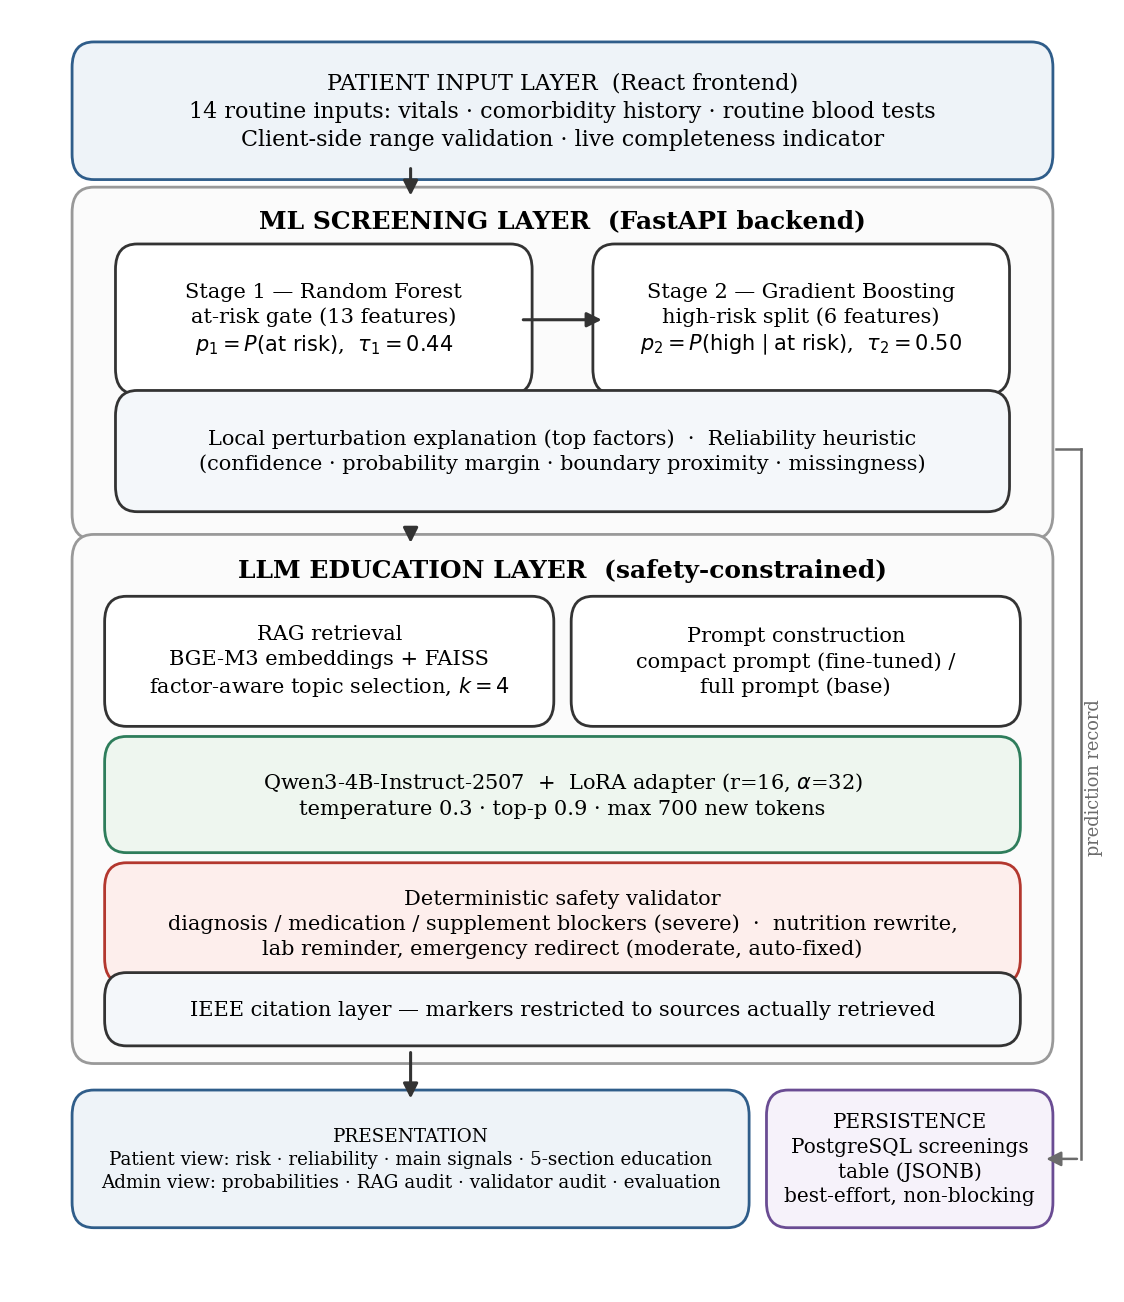
\includegraphics[width=0.92\textwidth]{fig_system_architecture.png}
\caption{Layered architecture of the proposed system. The screening layer
decides the risk category; the education layer may only explain it. Every
generated output passes the deterministic validator before delivery.}
\label{fig:architecture}
\end{figure}

The \textbf{input layer} collects fourteen routine measurements through a web
form with client-side range validation and a live completeness indicator, and
submits them to the backend.

The \textbf{screening layer} converts the submitted values into a feature
vector, applies the two-stage cascade, and produces the risk category, the class
probabilities, a per-feature attribution of the decision, and a reliability
assessment.

The \textbf{education layer} converts that structured output into patient-facing
text. It retrieves guideline passages selected according to the individual's
attributed risk factors, constructs a prompt containing the screening result,
the patient's own values and the retrieved passages, generates five labelled
sections with a fine-tuned language model, and then subjects the result to the
deterministic validator and a citation layer.

The \textbf{persistence layer} records each screening in a PostgreSQL table for
research use. It is deliberately best-effort: a database failure is logged and
skipped, never propagated to the user-facing request.

\section{Formal Model of the Screening Cascade}
\label{sec:cascade_model}

Let $x \in \mathcal{X}$ denote the feature vector of one individual, where
$\mathcal{X}$ is the space of the fourteen routine inputs enumerated in
Chapter~\ref{ch:methodology}. Let $\mathcal{Y} = \{\text{low}, \text{moderate},
\text{high}\}$ be the screening categories.

Rather than learning a single mapping $\mathcal{X} \rightarrow \mathcal{Y}$, the
system learns two binary probabilistic classifiers arranged in a cascade, shown
in Figure~\ref{fig:cascade}.

\begin{figure}[H]
\centering
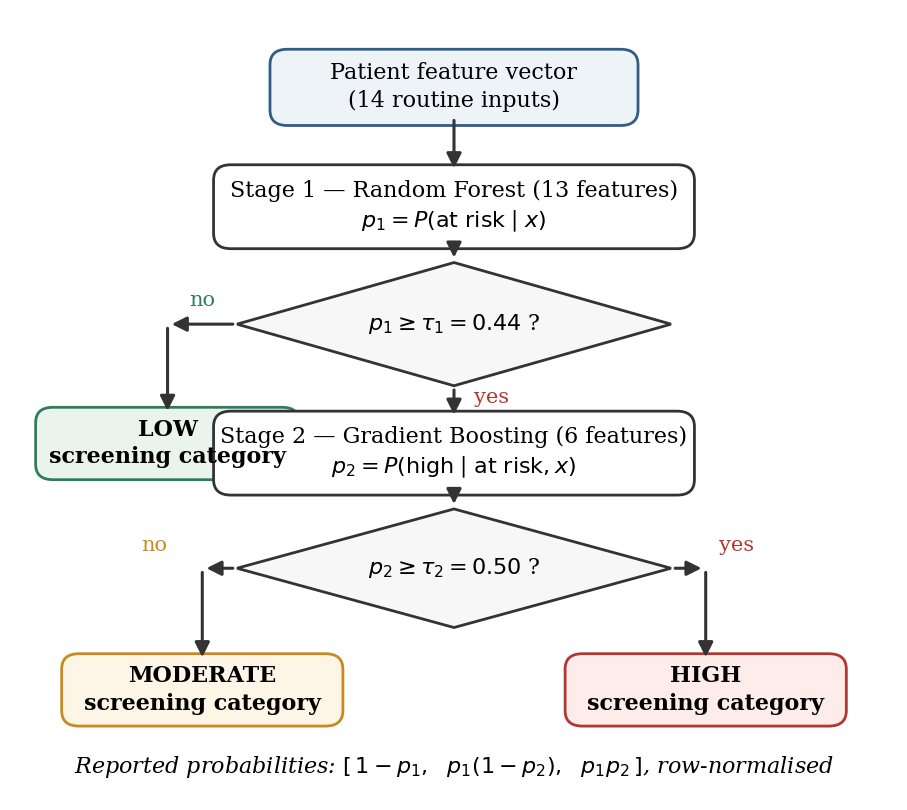
\includegraphics[width=0.66\textwidth]{fig_cascade.png}
\caption{Two-stage cascade. Stage~1 gates on the probability of being at risk;
only gated cases reach Stage~2, which separates high from moderate.}
\label{fig:cascade}
\end{figure}

\subsection{Stage 1: the at-risk gate}

Stage~1 is a binary classifier $f_1$ trained to separate the low category from
the union of moderate and high. Writing $S_1 \subset \mathcal{X}$ for the
13-feature subspace used by this stage,
\begin{equation}
\pone = f_1(x_{S_1}) = P(\text{at risk} \mid x), \qquad
\text{at risk} \equiv y \in \{\text{moderate}, \text{high}\} .
\label{eq:stage1}
\end{equation}

A decision threshold $\tauone$ gates the cascade:
\begin{equation}
g(x) = \mathbf{1}\!\left[\pone \geq \tauone\right], \qquad \tauone = 0.44 .
\label{eq:gate}
\end{equation}

Because $\tauone$ alone determines whether an individual can ever be assigned a
non-low category, it is the architectural control point for the asymmetric error
described in principle~2. Lowering $\tauone$ increases sensitivity to at-risk
individuals at the cost of more false referrals; the value $0.44$ was selected
on development data as described in Section~\ref{sec:threshold}.

\subsection{Stage 2: the high-risk discriminator}

Stage~2 is a second binary classifier $f_2$, trained on the at-risk subpopulation
to separate high from moderate, using a six-feature subspace $S_2$:
\begin{equation}
\ptwo = f_2(x_{S_2}) = P(\text{high} \mid \text{at risk}, x).
\label{eq:stage2}
\end{equation}

\subsection{Composition}

The predicted category is
\begin{equation}
\hat{y} =
\begin{cases}
\text{low}, & \text{if } \pone < \tauone,\\[2pt]
\text{high}, & \text{if } \pone \geq \tauone \ \text{and}\ \ptwo \geq \tautwo,\\[2pt]
\text{moderate}, & \text{otherwise},
\end{cases}
\qquad \tautwo = 0.50 .
\label{eq:decision}
\end{equation}

Applying the chain rule of probability, the three class probabilities reported to
the user are
\begin{align}
\tilde{P}(\text{low} \mid x)      &= 1 - \pone, \label{eq:plow}\\
\tilde{P}(\text{moderate} \mid x) &= \pone\,(1 - \ptwo), \label{eq:pmod}\\
\tilde{P}(\text{high} \mid x)     &= \pone\,\ptwo, \label{eq:phigh}
\end{align}
normalised so that they sum to unity:
\begin{equation}
P(c \mid x) = \frac{\tilde{P}(c \mid x)}{\sum_{c' \in \mathcal{Y}} \tilde{P}(c' \mid x)} .
\label{eq:normalise}
\end{equation}
The reported confidence is $\max_{c} P(c \mid x)$.

Note that $\ptwo$ is evaluated for every individual, but enters the decision in
Equation~\ref{eq:decision} only when the gate is open. This keeps the reported
probability vector well defined for all inputs while preserving the gating
semantics.

\section{Local Explanation Model}
\label{sec:explanation_model}

To make each prediction interpretable, the system attributes the decision to
individual inputs by single-feature perturbation against a fixed clinical
reference. Let $\hat{y}$ be the predicted category, $P(\hat{y} \mid x)$ the
corresponding probability from Equation~\ref{eq:normalise}, and $r_f$ a fixed
reference value for feature $f$. Define $x^{(f \rightarrow r_f)}$ as the input
$x$ with feature $f$ replaced by $r_f$ and all other features unchanged. The
contribution of $f$ is
\begin{equation}
\phi_f = P(\hat{y} \mid x) - P\!\left(\hat{y} \mid x^{(f \rightarrow r_f)}\right).
\label{eq:phi}
\end{equation}

A positive $\phi_f$ means the individual's actual value \emph{supports} the
predicted category relative to the reference; a negative value means it pulls
away from it. Features are ranked by $|\phi_f|$ and the largest are surfaced.

Two properties should be stated plainly. Each perturbed input is re-scored
through the complete cascade, so $\phi_f$ reflects genuine model behaviour
rather than a surrogate approximation. However, because exactly one feature is
varied at a time, $\phi_f$ does not capture interactions: for correlated
features the sum of individual contributions need not equal the effect of
changing them jointly. The method is therefore reported as model-agnostic local
perturbation, not as a Shapley attribution.

\section{Reliability Model}
\label{sec:reliability_model}

Not every prediction deserves equal trust. The system computes a deterministic
reliability level from three signals. Let $P_{(1)} \geq P_{(2)} \geq P_{(3)}$ be
the sorted class probabilities. Define the confidence $c = P_{(1)}$, the margin
\begin{equation}
m = P_{(1)} - P_{(2)},
\label{eq:margin}
\end{equation}
and let $n_{\mathrm{miss}}$ be the number of inputs the user left blank, which
the fitted preprocessing pipeline imputed. A prediction is considered near the
decision boundary when
\begin{equation}
\left|\pone - \tauone\right| \leq 0.06 \quad\text{or}\quad m < 0.15 .
\label{eq:boundary}
\end{equation}

The reliability level is then
\begin{equation}
\mathrm{rel} =
\begin{cases}
\text{low}, & n_{\mathrm{miss}} \geq 5 \ \lor\ c < 0.50 \ \lor\ m < 0.08,\\[2pt]
\text{moderate}, & \text{boundary} \ \lor\ c < 0.65 \ \lor\ n_{\mathrm{miss}} \geq 2,\\[2pt]
\text{high}, & \text{otherwise.}
\end{cases}
\label{eq:reliability}
\end{equation}

The three conditions encode three distinct failure modes: an input-starved
prediction leaning on imputation, a prediction made without conviction, and a
prediction that a small perturbation could flip. The rule is deterministic and
fully inspectable; it is a transparency device and is explicitly \emph{not} a
calibrated uncertainty quantification.

\section{Education Layer Model}
\label{sec:education_model}

The education layer is a function
\begin{equation}
E : (\hat{y},\, P(\cdot \mid x),\, \{\phi_f\},\, \mathrm{rel},\, x) \longrightarrow
\mathcal{S},
\end{equation}
where $\mathcal{S}$ is the space of five-section structured education documents
with the fixed section set
\[
\{\text{Summary},\ \text{Food habits},\ \text{Rest and sleep},\
\text{Daily routine},\ \text{Follow-up reminder}\}.
\]

$E$ is realised as a composition of four operators:
\begin{equation}
E = V \circ G \circ \Pi \circ R,
\label{eq:composition}
\end{equation}
where $R$ is factor-aware retrieval, $\Pi$ is prompt construction, $G$ is
language-model generation, and $V$ is the deterministic safety validator. The
ordering matters: $V$ is applied last and unconditionally, so no property
established by $V$ can be undone by $G$.

\subsection{Retrieval operator}

Let $\mathcal{K}$ be the knowledge base of guideline passages, each carrying a
topic tag $t(\kappa)$ and a restriction flag. Retrieval builds a query $q$ from
the risk category and the highest-ranked attributed factors, embeds it, and
returns $k$ passages. Rather than taking the top $k$ by similarity alone,
$R$ derives an ordered priority topic list $T(x)$ from the factors that
\emph{raise} the individual's risk, and selects the best-scoring passage for
each topic in turn before filling remaining slots by score. This guarantees that
the retrieved evidence reflects the individual's own dominant risk drivers
rather than the generic centroid of the corpus, and is what makes two
individuals in the same category receive different grounding.

\subsection{Safety validator model}

The validator is a function $V : \mathcal{T} \times \mathcal{C} \rightarrow
\mathcal{T} \times \Sigma$ mapping a candidate text and a context to a delivered
text and a status $\sigma \in \{\text{pass}, \text{sanitized}, \text{fallback}\}$.
It applies an ordered set of detectors, each classified by severity, as shown in
Figure~\ref{fig:validator}.

\begin{figure}[H]
\centering
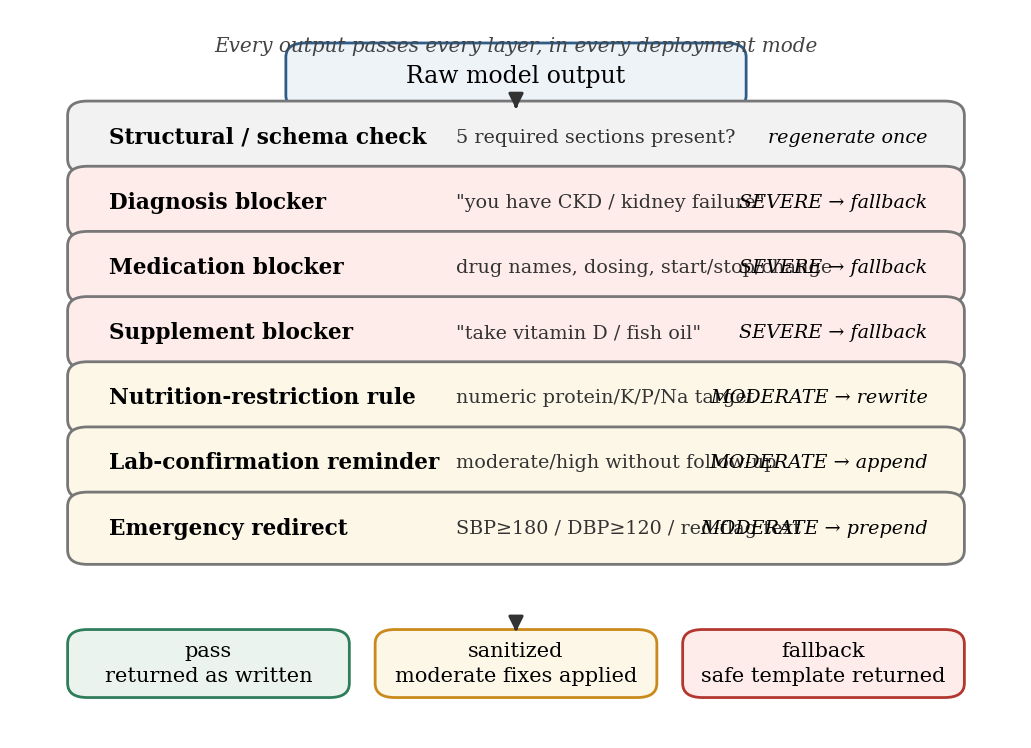
\includegraphics[width=0.82\textwidth]{fig_validator.png}
\caption{Layered safety validator. Severe violations replace the output with a
safe template; moderate violations are repaired in place; the structural check
triggers a single regeneration attempt.}
\label{fig:validator}
\end{figure}

Formally, write $w$ for the candidate text and $C$ for the request context, and
let $D_{\mathrm{sev}}$ and $D_{\mathrm{mod}}$ be the severe and moderate
detector families. Then
\begin{equation}
V(w, C) =
\begin{cases}
(w_{\mathrm{safe}},\ \text{fallback}), & \exists\, d \in D_{\mathrm{sev}} : d(w) = 1,\\[3pt]
(\rho(w, C),\ \text{sanitized}), & \exists\, d \in D_{\mathrm{mod}} : d(w) = 1,\\[3pt]
(w,\ \text{pass}), & \text{otherwise,}
\end{cases}
\label{eq:validator}
\end{equation}
where $\rho$ is the repair operator (rewriting numeric dietary targets into a
dietitian referral, appending the laboratory-confirmation reminder, or
prepending urgent-care redirection) and $w_{\mathrm{safe}}$ is a
fixed, condition-aware safe template.

The guarantee this provides is bounded but precise: for every unsafe pattern in
$D_{\mathrm{sev}} \cup D_{\mathrm{mod}}$, no text exhibiting that pattern can be
delivered, regardless of what the generative model produced. The guarantee does
not extend to patterns outside the detector set, a limitation examined in
Chapter~\ref{ch:discussion}.

\section{End-to-End Request Algorithm}
\label{sec:algorithm}

Algorithm~\ref{alg:pipeline} states the complete request path, and
Figure~\ref{fig:pipeline} shows it schematically.

\begin{figure}[H]
\centering
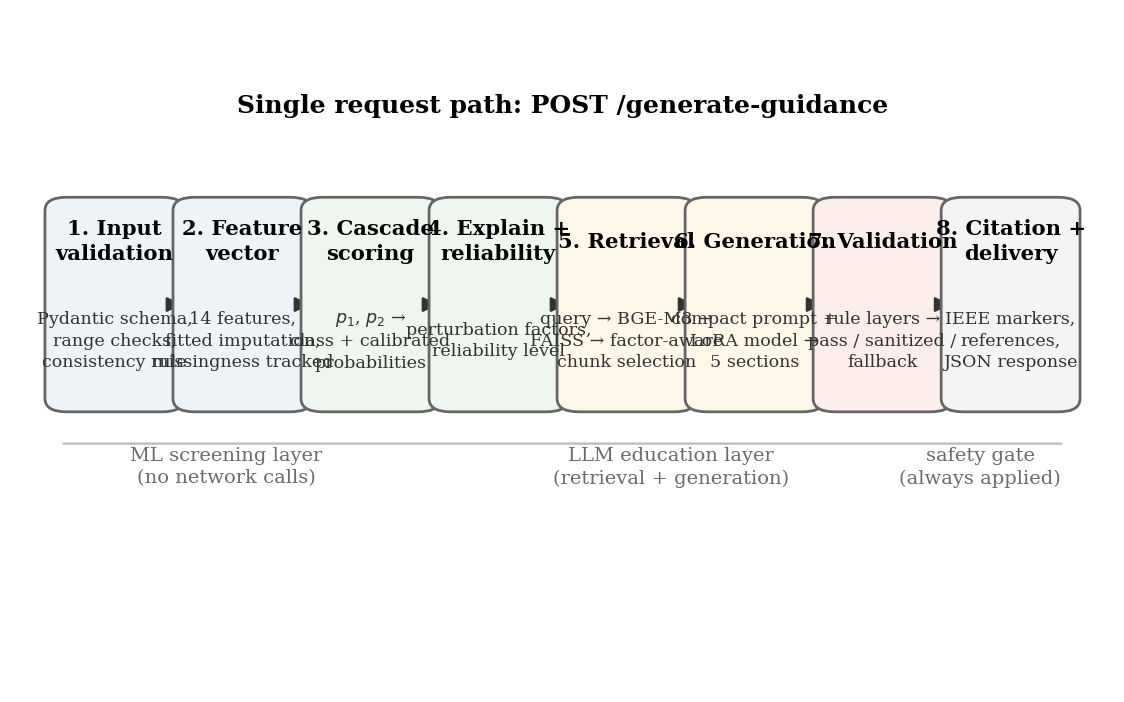
\includegraphics[width=\textwidth]{fig_pipeline_flow.png}
\caption{End-to-end request pipeline for a single screening, from input
validation through to the delivered, cited education document.}
\label{fig:pipeline}
\end{figure}

\begin{algorithm}[H]
\caption{End-to-end kidney-risk screening and education}
\label{alg:pipeline}
\begin{algorithmic}[1]
\Require Submitted measurements $u$; cascade $(f_1, f_2, \tauone, \tautwo)$;
knowledge base $\mathcal{K}$; language model $G$; validator $V$
\Ensure Risk category $\hat{y}$, delivered education document $s$, status $\sigma$
\State $u \gets \textsc{ValidateSchema}(u)$ \Comment{reject out-of-range / unknown fields}
\State $x \gets \textsc{BuildFeatureVector}(u)$ \Comment{consistency rule; missing $\rightarrow$ NaN}
\State $n_{\mathrm{miss}} \gets |\{f : x_f = \text{NaN}\}|$
\State $\pone \gets f_1(x_{S_1})$; \quad $\ptwo \gets f_2(x_{S_2})$
  \Comment{fitted imputation inside each stage}
\If{$\pone < \tauone$} \State $\hat{y} \gets \text{low}$
\ElsIf{$\ptwo \geq \tautwo$} \State $\hat{y} \gets \text{high}$
\Else \State $\hat{y} \gets \text{moderate}$
\EndIf
\State $P(\cdot \mid x) \gets \textsc{Normalise}(1-\pone,\ \pone(1-\ptwo),\ \pone \ptwo)$
\For{each supplied feature $f$ with reference $r_f$}
  \State $\phi_f \gets P(\hat{y} \mid x) - P(\hat{y} \mid x^{(f \rightarrow r_f)})$
    \Comment{re-scores the full cascade}
\EndFor
\State $\Phi \gets$ top features by $|\phi_f|$
\State $\mathrm{rel} \gets \textsc{Reliability}(P(\cdot\mid x), \pone, n_{\mathrm{miss}})$
\State $T \gets \textsc{PriorityTopics}(\Phi)$ \Comment{risk-raising factors first}
\State $q \gets \textsc{BuildQuery}(\hat{y}, \Phi)$
\State $\mathcal{R} \gets \textsc{FactorAwareRetrieve}(q, T, \mathcal{K}, k)$
\State $\pi \gets \textsc{BuildPrompt}(\hat{y}, P(\cdot\mid x), \Phi, \mathrm{rel}, x, \mathcal{R})$
\State $w \gets G(\pi)$
\If{$\neg\,\textsc{StructureOK}(w)$}
  \State $w \gets G(\pi \,\|\, \text{format reminder})$ \Comment{single retry}
\EndIf
\State $(s, \sigma) \gets V(w, \textsc{Context}(x, \hat{y}))$
\State $s \gets \textsc{AttachCitations}(s, \mathcal{R})$
  \Comment{markers restricted to retrieved sources}
\State \textsc{PersistBestEffort}$(u, \hat{y}, P, s, \sigma)$
\State \Return $(\hat{y}, s, \sigma)$
\end{algorithmic}
\end{algorithm}

Three ordering properties of Algorithm~\ref{alg:pipeline} are load-bearing.
First, the risk category is fixed at line 10, before any language-model
involvement, so generation cannot influence classification. Second, the
validator at line 23 is applied to whatever text generation produced, including
the retry, so the safety properties hold unconditionally. Third, citations are
attached at line 24 \emph{after} validation, drawing only on the passages
actually retrieved at line 18, which makes a fabricated citation structurally
impossible.
